\documentclass[a4paper]{scrartcl}
\usepackage[latin1]{inputenc}			% Für Umlaute
\usepackage[T1]{fontenc}			% Für richtige Schrift
\usepackage[ngerman]{babel}			% Für neue deutsche Rechtschreibung (Trennung)
\usepackage{color}
\usepackage{amsmath}
\usepackage{amssymb}
\usepackage{graphicx}
\usepackage{textcomp}				% Fürs Gardzeichen

\usepackage{scrpage2}				% Für Kopf- und Fußzeilen
\pagestyle{scrheadings}				% Für Kopf- und Fußzeilen
\clearscrheadfoot					% Für Kopf- und Fußzeilen


\begin{document}
\titlehead{Wintersemester 2017/2018\\Motion Planning\\Prof. Horsch, Rudi Scheitler}
\author{David Welsch, Ken Hasenbank}
\title{Praktikum 4 - Probabilistic Roadmap (PRM) - Nachbesserung}
\maketitle

\section*{Beschreibung der Aufgabe}

Das Ziel dieses Praktikums war es, auf Basis einer PRM einen Weg zwischen einer Start- und einer Zielkonfiguration zu finden. \\

Das Konzept von PRM ist es, eine bestimmte Anzahl an zufälligen Konfigurationen in den vorher definierten Konfigurationsraum zu streuen und diese auf Kollisionen zu testen. Ist der Punkt kollisionsfrei, so wird er als gültige Konfiguration gespeichert. Ist die definierte Anzahl an Konfigurationen erstellt und getestet, wird versucht, diese Konfigurationen durch kollisionsfreie Pfade zu verbinden. So entsteht einer oder mehrere Graphen, welche alle gültigen Konfigurationen beinhalten. Nun müssen noch die Start- sowie  Zielkonfiguration zu den Graphen hinzugefügt werden. Liegen Start- und Zielkonfiguration auf demselben Graphen kann mittels eines Graphen-Such-Algorithmus wie beispielsweise dem A* oder Dijkstra ein Pfad von Start- zu Zielkonfiguration gefunden werden. Die Punkte auf diesem Pfad beschreiben alle Konfigurationen, die benötigt werden, um die Bewegung auszuführen.\\

Als Resampling-Algorithmus nutzen wir die Gaußschen-Sampling Methode. Wie in Abbildung \ref{img:GausSample} zu sehen, werden hier hauptsächlich Nodes in der Nähe von Obstacles erstellt. Damit weitere Verbindungen möglich sind, erstellen wir in jedem Resampling Schritt zusätzlich eine kleine Zahl zufällige Nodes.\\

\begin{figure}
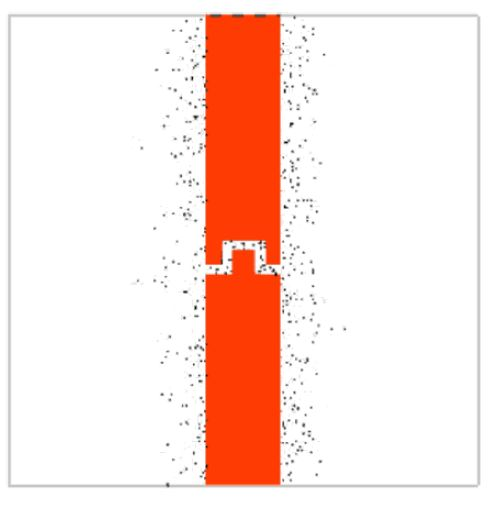
\includegraphics[width=\textwidth]{GaussianSamplingNodeDistribution.JPG}
\caption{Gaußsches Samplingverfahren - Node-distribution (aus dem Skript)}
\label{img:GausSample}
\end{figure}

In der gegebenen Aufgabe soll ein Wurm mit 5 Freiheitsgraden (zwei davon translatorisch, drei rotatorisch) durch einen Parcours mit 5 Hindernissen bewegt werden.

\section*{Beschreibung der L"osung}

Zur L"osung haben wir den vorgegeben Code-Rahmen verwendet. Alle Berechnungen erfolgen in der Datei \textit{main.cpp} und dort in der Methode \textit{\_tmain}. Wir nutzen zudem eine Methode um die Kanten zum Graphen hinzuzufügen. Diese haben wir ausgelagert, da wir die Erstellung zur schnelleren Bearbeitung parallelisiert haben.\\

Zudem gibt es zwei Methoden, welche zufällige (\textit{buildRandomNodes}) beziehungsweise nach dem Guaßschen Sampling-Verfahren (\textit{resampling}) Nodes zum rtree hinzufügt.\\

Ab hier wird durch die Beschreibung der Datei \textit{main.cpp} unser Vorgehen erläutert:

\begin{itemize}
	\item (Zeilen 29-55) In diesen Zeilen befindet sich die Methode \textit{addEdges}. Diese fügt zum übergebenen Graphen \textit{g} kollisionsfreie Kanten hinzu.\\
	Die übergebenen Parameter haben folgende Funktionen:
	\begin{itemize}
		\item \textit{int num}: Dieser Parameter wird verwendet, um beim debuggen die Threadnummer zu erkennen
		\item \textit{int start}: Mit diesem Parameter wird definiert, ab welcher Konfiguration im Graphen begonnen werden soll.
		\item \textit{int end}: Mit diesem Parameter wird definiert, bis zu welcher Konfiguration im Graphen die Berechnung durchgeführt werden soll.
		\item \textit{graph\_t \&g}: Dieser Parameter enthält eine Referenz auf den Graphen, welcher später alle Verbindungen zwischen den Konfigurationen enthalten soll. Es wird eine Referenz übergeben, da später mehrere Threads auf diesen Graphen schreiben und durch die Übergabe als Kopie nur die Änderungen eines Threads übernommen werden würden.
		\item \textit{knn\_rtree\_t \&rtree}: Dieser Parameter enthält den rtree, welcher zur Bestimmung der \textit{x} nächsten Konfigurationen benötigt wird. Dieser wird als Referenz übergeben, damit die Änderungen später direkt abrufbar sind und nicht zurückgegeben werden müssen.\\
	\end{itemize}
	Im Folgenden wird nun die Methode selbst beschrieben. Die Zeilenangaben sind absolut in der Datei \textit{main.cpp} angegeben.
	\begin{itemize}
		\item (Zeile 33) Hier wird die for-Schleife gestartet, welche von der übergebenen Start- bis zur Zielkonfiguration läuft.
		\item (Zeilen 34-36) Zur Kontrolle, ob die Berechnung noch läuft, wird bei jedem 500sten Durchlauf ein . auf der Konsole ausgegeben.
		\item (Zeile 37-41) Hier wird zuerst die aktuell untersuchte Konfiguration geladen (Variable \textit{actVector}). Dann wird ein neuer std::vector erstellt, welcher die benachbarten Konfigurationen aus dem rtree speichert. In Zeile 40 wird dann ein Roboter in Form des 5-dimensionalen Wurms erstellt, welcher die aktuell zu untersuchende Konfiguration annimmt. In Zeile 41 werden schließlich mit Hilfe des rtrees die nächsten 10 Nachbarn der aktuell zu untersuchenden Konfiguration gesucht und in den std::vector \textit{nearest} gespeichert. 
		\item (Zeile 44-55) In diesen Zeilen wird getestet, welche der gefundenen Nachbarn kollisionsfrei von der aktuell untersuchten Konfiguration erreicht werden können. Hierzu wird mit einer weiteren for-Schleife jede Nachbarkonfiguration mittels \textit{cell.CheckMotion} die Bewegung von der aktuellen Konfiguration (aus der übergeordneten for-Schleife) zur gefundenen Nachbarkonfiguration getestet. Zudem wird überprüft, ob es die Kante bereits gibt, da sie dann nicht erneut überprüft werden muss. Ist sie nicht vorhanden und die Bewegung ist kollisionsfrei möglich, wird die Kante inklusive zugehöriger Länge dem Graphen \textit{g} hinzugefügt (Zeile 49).
		\item Daraufhin wird noch die Node in die Liste eingefügt, die später beim resampling verwendet wird, sollte mindest eine Verbindung fehlgeschlagen sein.
	\end{itemize}
	Damit ist die Methode \textit{addEdges} beschrieben.\\
	
	\item Die im folgenden beschriebene Methode \textit{resample}. Diese haben wir in der Nachbesserung implementiert, um neue Nodes nach dem \textit{Gaussian Sampling}-Verfahren zu erstellen. Dieses Verfahren funktioniert wie folgt:
	\begin{enumerate}
		\item Ein zufälliger Punkt im Konfigurationsraum wird gesucht.
		\item Ein zweiter Punkt wird durch Gaussche Normalverteilung im Umkreis des vorher zufällig erstellten Punkts gesucht.
		\item Wenn beide kollidieren oder beide im Freiraum sind werden sie verworfen.
		\item Ist einer der beiden Punkte im Freiraum, der andere kollidiert jedoch, wird der Punkt im Freiraum behalten.
	\end{enumerate} 
	Durch dieses Verfahren werden nur Nodes aufgenommen, welche innerhalb des vorher definierten Radius um ein Objekt herum sind. Bei der Anwendung dieses Verfahrens ist darauf zu achten, dass der Radius nicht zu groß gewählt wird, da ansonsten auch Punkte weit weg von Objekten erfasst werden. Wird der Radius jedoch zu klein gewählt, ist die Wahrscheinlichkeit, dass zwei Punkte gefunden werden, von denen einer im Freiraum liegt, der andere jedoch nicht, sehr gering. Dieser Radius wurde von uns experimentell auf \textit{0,07} für die translatorischen und \textit{1,00} für die rotatorischen Freiheitsgrade ermittelt.\\
	
	Im Folgenden wird nun unsere Implementierung kurz erläutert. Die Erläuterung bezieht sich auf die Zeilen 68 bis 116 im Code.
	
	\begin{itemize}
		\item Die Methode ist so implementiert, dass sie so lange läuft, bis zu allen Nodes, welche mindestens eine fehlgeschlagene Verbindung haben, geresamplt wurde.
		\item Zu Beginn wird der Vektor aus der Liste gelesen.
		\item In Zeile 76 wird eine for-Schliefe initialisiert, welche so oft durchlaufen wird, wie es fehlgeschlagene Verbindungen bei dieser Node gegeben hat.
		\item In dieser wird zuerst ein double-Array erstellt, in welchem die zufälligen Werte des neuen Vektors gespeichert werden.
		\item In der for-Schleife in den Zeilen 80 bis 91 wird durch die Gaußsche Normalverteilung, welche in der boost-Library bereits implementiert ist, für jeden Freiheitsgrad ausgehend vom aus der Liste gelesenen Vektor mit dem oben angegebenen Radius ein neuer Wert erstellt.
		\item Anschließend wird der Vektor zusammen gebaut.
		\item Dann folgt die Plausibilitätsüberprüfung. Zusätzlich zu der im Verfahren genannten Prüfungen wird hier außerdem überprüft, ob der neue Vektor noch im CSpace liegt. Ansonsten wird er verworfen.
		\item Zum Schluss wird die erstellte Node noch in den rtree eingefügt und der Zähler der erstellten Nodes erhöht.
		\item Sind alle Nodes abgearbeitet, wird die Anzahl der erstellten neuen Nodes zurückgegeben.
	\end{itemize}
	
 	Damit ist die Methode resampling abgeschlossen.
	
	\item Methode \textit{buildRandomNodes}: In dieser Methode werden eine bestimmte Anzahl an zufälligen, kollisionsfreien Nodes erstellt. Dieser Schritt wird zu Beginn des Algorithmus und bei jedem Resampling-Schritt mit geringerer Anzahl an Nodes durchgeführt.
	\begin{itemize}
		\item Es wird eine while-Schleife begonnen, welche so lange läuft, bis die angegebene Zahl an Nodes erstellt wurde.
		\item (Zeilen 118-126) In diesen Zeilen  wird zuerst eine zufällige, kollisionsfreie Konfiguration erstellt und diese dem rtree hinzugefügt. 
	\end{itemize}
	
	\item Methode \textit{\_tmain}: Im Folgenden wird die Methode \textit{\_tmain} beschrieben, welche die Berechnung entsprechend des PRM durchführt. 
	
	\begin{itemize}
		\item (Zeilen 136-223) In diesen Zeilen werden die Testcases sowie benötigte Variablen deklariert.
		\item (Zeilen 225-227) Hier werden DWORDs definiert, welche Zeitstempel speichern, um die benötigte Zeit zur Berechnung der einzelnen Schritte sowie der gesamten Berechnungszeit anzeigen zu können.
		\item (Zeile 229) In dieser Zeile wir der Graph initialisiert, welcher später die Lösung enthält.
		\item (Zeilen 231-233) In diesen Zeilen werden benötigte Variablen zum Resampling initialisiert. Die Verwendung dieser Variablen wird später erläutert.
		\item (Zeilen 238-255) In den folgenden if-Abfragen wird geprüft, ob sowohl Start- als auch Zielkonfiguration kollisionsfrei sind. Ist dies nicht der Fall, wird das Programm direkt terminiert, da kein gültiger Pfad erstellt werden kann.
		\item (Zeile 258) Hier wird eine do-while Schleife gestartet, um das Resampling zu realisieren.
		
		\item (Zeilen 260-262) Diese Zeilen dienen dazu, die Zeit des ersten Schrittes zu erfassen, sowie während dem Programmlauf zu sehen, an welcher Stelle sich das Programm befindet. Außerdem wird die Variable \textit{resamplesDone} hochgezählt, um zu erfassen, wie oft bereits neue Konfigurationen (Nodes) und Verbindungen zwischen diesen (Edges) erstellt wurden.
		
		\item (Zeilen 265-273) Hier wird je nachdem, ob es der erste Durchlauf oder ein Resampling-Durchlauf ist, entweder nur zufällige Nodes oder Nodes per resampling erstellt.
		
		\item (Zeilen 276-286) Diese Zeilen dienen dazu, die Zeit des ersten Schrittes auszugeben sowie die Zeitmessung für den neuen, zweiten Schritt zu starten.
		\item (Zeilen 287-295) Hier werden acht Threads erstellt, welche die Berechnung der Edges mit Hilfe der Methode \textit{addEdges} von oben durchführen.
		\item (Zeilen 295-311) Anschließend werden wieder Ausgaben erstellt, welche zur Laufzeit aufzeigen, wie viele Edges erstellt wurden, sowie die benötigte Zeit des zweiten Schrittes ausgeben.
		\item (Zeile 312) Wird nicht geresampled, (entpricht dem ersten Durchgang), wird in den folgenden Zeilen die Startkonfiguration dem rtree hinzugefügt. (Zeilen 313-317)
		\item (Zeile 320-334) In diesen Zeilen wird genau wie in der Methode \textit{addEdges} die nächsten Nachbarn gesucht (hier jedoch die nächsten 500, um sicher eine Verbindung von Start-Konfiguration zu einem der entstandenen Graphen zu finden.)
		\item (Zeilen 335-347) Wieder zur Information
		\item (Zeilen 348-370) Anschließend wird genau wie mit der Startkonfiguration auch mit der Zielkonfiguration verfahren.
		\item (Zeilen 379-383) In diesen Zeilen wird auf der Konsole der aktuelle Zustand des Graphen ausgegeben. Diese Informationen beinhalten die Anzahl der Konfigurationen, sowie die Anzahl der Verbindungen zwischen diesen. Zudem wird die Anzahl der nicht zusammenhängenden Graphen ausgegeben.
		\item (Zeilen 384-388) Hier wird getestet, ob sich die Start- und Zielkonfiguration auf demselben Graphen befinden. Ist dies nicht der Fall, wird die Variable \textit{resampling} auf true gesetzt, damit im weiteren Verlauf klar ist, dass geresampled werden soll. Zudem wird ausgegeben, dass keine Verbindung gefunden werden konnte.
		\item (Zeilen 389-393) Sollten beide Konfigurationen auf demselben zusammenhängenden Teil des Graphen liegen, wird die Variable \textit{resampling} auf false gesetzt, da eine Verbindung der Start- und Zielkonfiguration möglich ist und ein resampling nicht mehr nötig ist. Zudem wird die Variable \textit{solutionFound} auf true gesetzt um anzuzeigen, dass eine Lösung möglich ist.
		\item (Zeilen 395-407) In diesen Zeilen wird der Nutzer ab 5 resamples gefragt, ob er einen weiteren Resampling-Durchlauf starten möchte oder die Ausführung des Programms erfolglos beenden möchte. Diese Abfrage haben wir eingebaut, um Endlosschleifen zu verhindern.
		\item (Zeilen 409-423) Hier werden wieder Informationen ausgegeben und die do-while Schleife geschlossen. Außerdem wird das Programm beendet, sollte trotz Resampling keine Lösung gefunden worden sein und der Nutzer die Ausführung des Programms abgebrochen haben.
		\item (Zeilen 425-430) Mit Hilfe der Implementierung des Dijkstra-Algorithmus in der Boost-Library wird der kürzeste Weg von der Start- zur Zielkonfiguration ermittelt. Dieser Weg ist zu diesem Zeitpunkt im Programm auf jeden Fall vorhanden, da ansonsten die Ausführung des Programms beendet worden wäre.
		\item (Zeile 432) Die Distanz zwischen Start- und Zielkonfiguration wird ausgegeben.
		\item (Zeile 435-443) Wieder Ausgaben zur Information
		\item (Zeile 445-450) Hier wird rückwärts (ausgehend von der Zielkonfiguration) durch den vom Dijkstra erstellten Pfad gelaufen, um den Weg von Start- zu Zielkonfiguration zu speichern.
		\item (Zeilen 452-462) Anschließend wird der erstellte Pfad mit Hilfe der gelieferten Methode \textit{write\_easyrob\_program\_file} in die Datei \textit{solution.prg} geschrieben und die letzten Zeitstempel ausgegeben.
		\item Die Methode \textit{write\_easyrob\_program\_file} haben wir so umgeschrieben, dass zum ersten Punkt direkt gesprungen wird, um unschöne Ausgaben in Easyrob zu verhindern.
	\end{itemize} 
\end{itemize}
	Damit endet die Datei \textit{main.cpp} und damit auch die Beschreibung unserer Lösung.
	
\section*{Was wir gelernt haben}

Die Implementierung hat Spass gemacht, da wir die Bewegungen des Wurms dann verfolgen konnten. Wir haben gelernt, dass die Parallelisierung der Verbindungsberechnung sehr große Vorteile bringt.

\end{document}